\documentclass[journal]{IEEEtran}
\usepackage[english]{babel}

\usepackage{amssymb, amsmath} %Paquetes matemáticos de la American Mathematical 
\usepackage[utf8]{inputenc}
\usepackage{graphicx}
\usepackage{float}
\usepackage{hyperref}
\usepackage{listings}
\usepackage[table, svgnames, dvipsnames]{xcolor}
\usepackage{multirow}
\usepackage{supertabular}
\usepackage{longtable}

\definecolor{codegreen}{rgb}{0,0.6,0}
\definecolor{codegray}{rgb}{0.5,0.5,0.5}
\definecolor{codepurple}{rgb}{0.58,0,0.82}
\definecolor{backcolour}{rgb}{0.95,0.95,0.92}
% Definicio de estilo para el codigo fuente que se cita
\lstdefinestyle{mystyle}{
    backgroundcolor=\color{backcolour},   
    commentstyle=\color{codegreen},
    keywordstyle=\color{magenta},
    numberstyle=\tiny\color{codegray},
    stringstyle=\color{codepurple},
    basicstyle=\ttfamily\footnotesize,
    breakatwhitespace=false,         
    breaklines=true,                 
    captionpos=b,                    
    keepspaces=true,
    numbers=left,                    
    numbersep=5pt,                  
    showspaces=false,                
    showstringspaces=false,
    showtabs=false,                  
    tabsize=2,
}
\lstset{style=mystyle}

\renewcommand{\lstlistingname}{Código}

\ifCLASSINFOpdf

\else

\fi
\begin{document}

\title{Ejercicio 10 - tema 7 \\ Administración de datos Undo}
%
\author{Vicente Romero Andrade}

\markboth{Ejercicio 10 - tema 7 Administración de datos Undo, Julio~2021}%
{Shell \MakeLowercase{\textit{et al.}}: }
% The only time the second header will appear is for the odd numbered pages

\maketitle


\IEEEpeerreviewmaketitle

\section{Objetivo}
% The very first letter is a 2 line initial drop letter followed

\IEEEPARstart{E}{l} objetivo es comprender e ilustrar los efectos que 
produce un tablespace undo sin espacio durante la operación de la base de datos.

\section{Desarrollo}
\subsection{Generar una sentencia SQL que muestre el tablespace undo que actualmente está en uso}
\begin{lstlisting}[language=sql, caption=sentencia consulta tablespace undo,label={lst:codigo1}]
SELECT value FROM v$parameter WHERE name='undo_tablespace';
\end{lstlisting}
\begin{figure}[H]
  \centering
  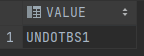
\includegraphics[scale=.75]{captura_1.png}
   \caption{Salida punto A}
   \label{fig:validador_1}
\end{figure}
\subsection{Generar una sentencia SQL que genere un nuevo tablespace 
undo cuya característica principal es contar con un espacio muy limitado y por lo tanto
la base de datos estará en riesgo de generar errores al requerir más espacio undo del disponible. 
Nombrar al tablespace undotbs2, asignarle un
solo data file ubicado en '/u01/app/oracle/oradata/<ORACLE\_SID>/undotbs\_2.dbf' 
con una capacidad únicamente de 30 MB. El data file no deberá auto extenderse. La administración de sus extensiones debe ser local}
\begin{lstlisting}[language=sql, caption=sentencia generar tablespace undo,label={lst:codigo2}]
create undo tablespace undotbs2
datafile '/u01/app/oracle/oradata/VRABDA2/undotbs_2.dbf' size 30M
autoextend off
extent management local autoallocate;
\end{lstlisting}
\subsection{Generar la sentencia SQL necesaria para que la instancia 
ahora haga uso del nuevo tablespace en lugar el actual. Aplicar el cambio únicamente
mientras la instancia esté iniciada}
\begin{lstlisting}[language=sql, caption=sentencia generar tablespace undo,label={lst:codigo2}]
alter system set undo_tablespace='UNDOTBS2' scope=memory;
\end{lstlisting}
\subsection{Crear una nueva sesión con el usuario SYS, 
ejecutar nuevamente la sentencia del inciso A para 
verificar que la instancia ahora está haciendo uso del tablespace undotbs2}
\begin{figure}[H]
  \centering
  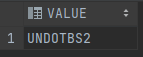
\includegraphics[scale=.75]{captura_2.png}
   \caption{Salida punto D}
   \label{fig:validador_2}
\end{figure}
\subsection{Considerar la vista v\$undostat. Generar la siguiente consulta. Mostrar la fecha inicio y fin del periodo de la muestra hasta nivel de segundos,
el id del tablespace que se está empleando, total de bloques undo empleados, total de transacciones, id de la consulta que tardó el mayor tiempo
en ejecutarse, tiempo en segundos de la consulta que más tiempo tardó en ejecutarse durante el periodo de la muestra, número de bloques undo
activos, no expirados y expirados; el valor del parámetro undo\_retention calculado por la instancia. Ordenar los registros con base a la fecha
de inicio de forma descendente. Mostrar únicamente los primeros 20 registros}
\begin{lstlisting}[language=sql, caption=sentencia consulta tablespace stats,label={lst:codigo2}]
SELECT BEGIN_TIME,
  END_TIME,
  UNDOTSN,
  UNDOBLKS as TOTAL_BLOQUES_UNDO_USADOS,
  TXNCOUNT as NUM_TRANSACCIONES,
  MAXQUERYID,
  MAXQUERYLEN,
  ACTIVEBLKS,
  UNEXPIREDBLKS,
  EXPIREDBLKS,
  TUNED_UNDORETENTION
FROM V$UNDOSTAT WHERE ROWNUM<=20 ORDER BY BEGIN_TIME DESC;
\end{lstlisting}
\begin{figure}[H]
  \centering
  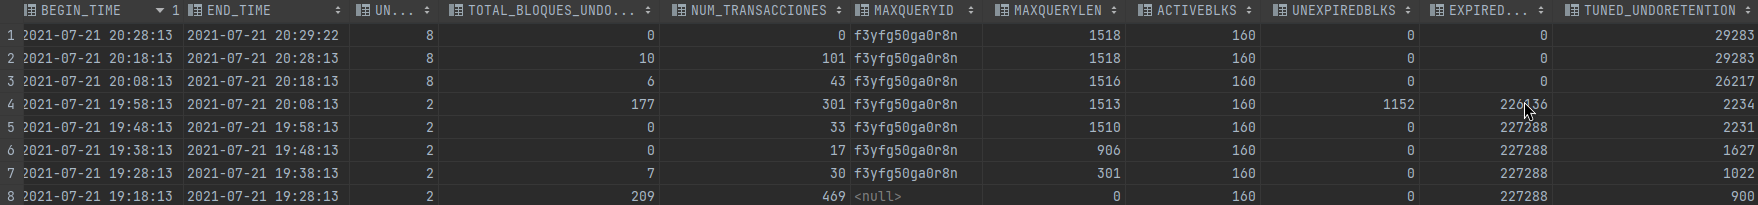
\includegraphics[scale=.14]{captura_3.png}
   \caption{Salida punto E}
   \label{fig:validador_3}
\end{figure}
\subsection{Considerar el periodo de muestreo más reciente de la consulta realizada en el inciso E}
\subsubsection{¿Cuantos bloques podrían ser sobrescritos sin causar mayores inconvenientes?}
Los que son EXPIRED pueden ser sobrescritos por lo tanto es 0 asi que ningun bloque se sobreescribira.
\subsubsection{¿Cuántos bloques NO pueden ser sobrescritos aun?}
160 bloques que corresponden a los activos

\subsection{Observar los valores de la columna undotsn de la consulta del inciso E. Confirmar 
que a partir del cambio del tablespace undo, el valor de esta columna cambia. Generar una sentencia 
SQL que permita mostrar los nombres de los tablespaces asociados a los valores de esta columna. 
Tip: auxiliarse de v\$tablespace. En la consulta incluir únicamente el periodo de la muestra, id del tablespace y su nombre}
\begin{lstlisting}[language=sql, caption=sentencia consulta tablespace id-nombre,label={lst:codigo3}]
SELECT BEGIN_TIME,
       END_TIME,
       UNDOTSN,
       T.NAME
FROM V$UNDOSTAT U JOIN V$TABLESPACE T ON U.UNDOTSN=T.TS# WHERE ROWNUM<=20 ORDER BY BEGIN_TIME DESC;
\end{lstlisting}
\begin{figure}[H]
  \centering
  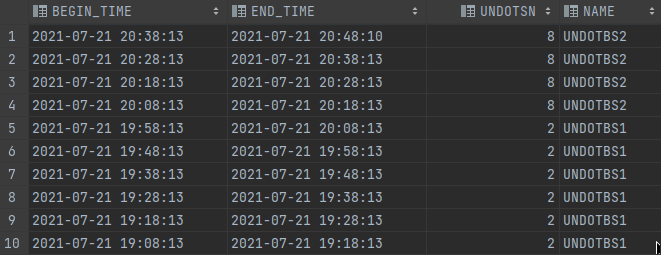
\includegraphics[scale=.30]{captura_4.png}
   \caption{Salida punto G}
   \label{fig:validador_4}
\end{figure}
\subsection{Generar una consulta que muestre las siguientes columnas: Nombre del tablespace undo que fue creado en pasos anteriores, total de bloques que
contiene, total de bloques libres, porcentaje de bloques libres. Confirmar que el porcentaje de bloques libres es bajo, menor al 20\%. Esta condición
pone en riesgo la operación correcta que requieren hacer uso de los datos Undo}
\begin{lstlisting}[language=sql, caption=sentencia consulta tablespace bloques libres,label={lst:codigo4}]
SELECT T.TABLESPACE_NAME,
  DF.BLOCKS TOTAL_BLOQUES,
  (DF.BLOCKS-SUM(E.BLOCKS)) BLOQUES_LIBRES,
  TRUNC(((DF.BLOCKS-SUM(E.BLOCKS))/DF.BLOCKS *100),2) PORCENTAJE_LIBRE FROM DBA_TABLESPACES T
JOIN DBA_DATA_FILES DF
   ON T.TABLESPACE_NAME=DF.TABLESPACE_NAME
JOIN DBA_UNDO_EXTENTS E
   ON T.TABLESPACE_NAME=E.TABLESPACE_NAME
WHERE T.TABLESPACE_NAME='UNDOTBS2'
GROUP BY T.TABLESPACE_NAME,DF.BYTES,DF.BLOCKS;
\end{lstlisting}
\begin{figure}[H]
  \centering
  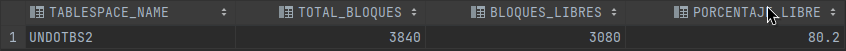
\includegraphics[scale=.28]{captura_5.png}
   \caption{Salida punto H}
   \label{fig:validador_5}
\end{figure}

\subsection{Empleando el usuario creado en temas anteriores, generar una tabla con la siguiente estructura}
\begin{lstlisting}[language=sql, caption=sentencia crear tabla,label={lst:codigo6}]
  DECLARE
  v_count number;
  v_count_s number;
  v_username varchar2(30) := 'VRA_TBS_MULTIPLE';
  v_table varchar2(30) := 'VRA_CADENA_2';
  v_secuencia varchar2(30) :='SEC_VRA_CADENA_2';
BEGIN
  --Verificar si la table existe
  select count(*) into v_count
  from all_tables
  where table_name = v_table
  and owner = v_username;

  --Verificar si la secuencia existe
  select count(*) into v_count_s
    from all_sequences
  where sequence_name = v_secuencia
    and sequence_owner = v_username;
  --Si existe la tabla, entonces se borra
  if v_count > 0 then
    execute immediate 'drop table '||v_username||'.'||v_table;
  end if;
  if v_count_s > 0 then
    execute immediate 'drop sequence '||v_username||'.'||v_secuencia;
  end if;
  execute immediate 'create table '||v_username||'.'||v_table||' (
    id number constraint vra_cadena_2_pk primary key,
    cadena varchar2(1024)
  ) nologging';
  execute immediate 'create sequence '||v_username||'.'||v_secuencia;
end;
/
-- Inserts
declare
  v_rows number;
  v_stmt varchar2(200);
  v_username varchar2(30) := 'VRA_TBS_MULTIPLE';
  v_table varchar2(30) := 'VRA_CADENA_2';
  v_secuencia varchar2(30) :='SEC_VRA_CADENA_2';
begin
v_rows := 50000;
v_stmt := 'insert into '||v_username||'.'||v_table||'(
  id, cadena
  ) values (:1, :2)';
for v_index in 1 .. v_rows loop
  execute immediate v_stmt using VRA_TBS_MULTIPLE.SEC_VRA_CADENA_2.nextval, dbms_random.string('P',1024);
end loop;
end;
/
commit;
\end{lstlisting}
\subsection{Replicación del error al ejecutar sentencias DML}
\begin{figure}[H]
  \centering
  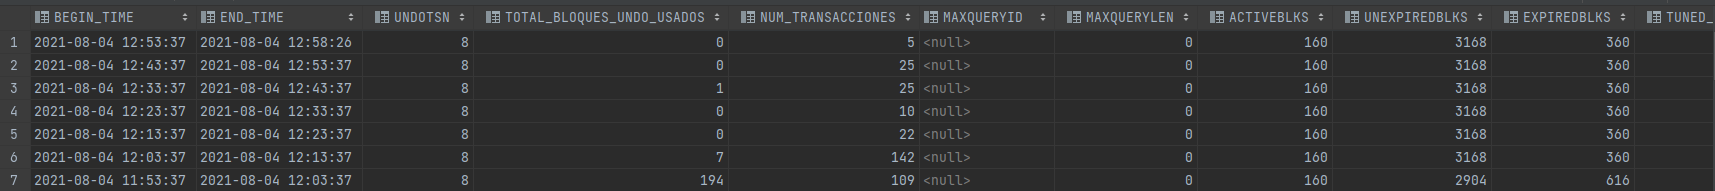
\includegraphics[scale=.14]{captura_6.png}
   \caption{Salida consulta punto E}
   \label{fig:validador_6}
\end{figure}
\begin{table}[H]
  \centering
  \resizebox{\linewidth}{!}{\begin{tabular}{|c|c|c|c|c|} 
   \hline
   Registros eliminados & \# bloques utilizados & \# transacciones ejecutadas & \#bloques activos & Retención en segundos calculado \\ [0.1ex] 
   \hline
   1 - 5000 & 835 & 138 & 160 & 9835 \\
   \hline
   5001 - 10000 & 1669 & 144 & 160 & 1896 \\
   \hline
   10001 - 15000 & 835 & 12 & 160 & 1741 \\
   \hline
  \end{tabular}}
  \caption{Tabla registros eliminados}
  \label{tabla:1}
\end{table}
\subsubsection{Revisar los datos de la tabla y generar una conclusión al respecto}
En este caso el unico cambio significativo es el tiempo de retención el cual fue bajando
\subsection{¿Qué acciones se pueden realizar para corregir el error adicional a aumentar el tamaño del tablespace undo?}
A parte de aumentar el tamaño de datafile que contiene el tablespace undo otra acción seria
configurar la cláusula $retention\ noguarantee$ sacrificando datos los datos unexpired.
\subsection{Replicación del error snapshoot too old}
\subsubsection{¿Cuántas instrucciones delete se tuvieron que ejecutar para provocar el error snapshppt too old?}
4 instrucciones
\begin{figure}[H]
  \centering
  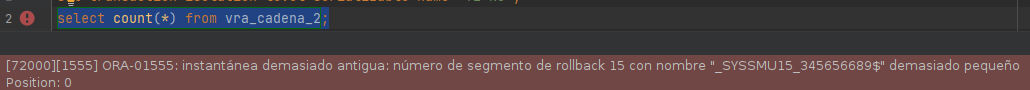
\includegraphics[scale=.23]{captura_7.png}
   \caption{Salida error snapshoot to old}
   \label{fig:validador_7}
\end{figure}
\subsection{Provocar ahora el comportamiento inverso: Hacer que la base de datos le de preferencia a consultas que requieran hacer uso de datos undo en lugar de dar preferencia a las sentencias SQL}
\subsubsection{Incluir la sentencia SQL que permite modificar este comportamiento, ejecutarla}
\begin{lstlisting}[language=sql, caption=Configuración priorizar datos undo,label={lst:codigo7}]
-- Se configura el retention guarantee
alter tablespace undotbs2 retention guarantee;
\end{lstlisting}
\begin{lstlisting}[language=sql, caption=script que se ejecuta constantemente para eliminar los datos y llenar undo,label={lst:codigo8}]
declare
  v_rows number;
  v_stmt varchar2(200);
  v_username varchar2(30) := 'VRA_TBS_MULTIPLE';
  v_table varchar2(30) := 'VRA_CADENA_2';
begin
  v_rows := 10;
  v_stmt := 'delete from '||v_username||'.'||v_table||'
    where id in (SELECT id from '||v_username||'.'||v_table||' WHERE ROWNUM<=5000)';
  execute immediate v_stmt;  
end;
/
commit;
\end{lstlisting}
\begin{figure}[H]
  \centering
  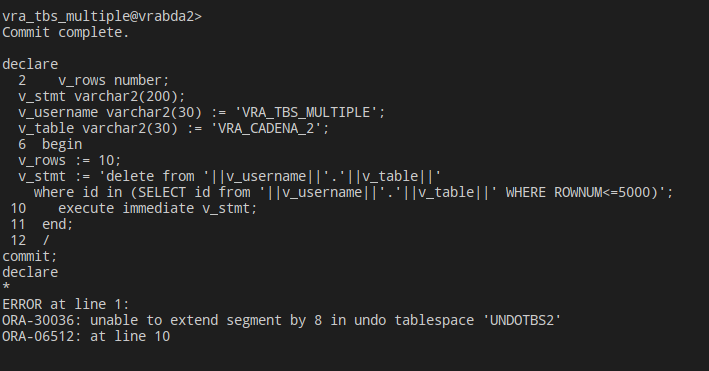
\includegraphics[scale=.23]{captura_8.png}
   \caption{Salida error comportamiento inverso}
   \label{fig:validador_8}
\end{figure}
\section{Conclusiones}
En este ejercicio se logro comprender mejor la administración de datos undo asi como lo que implican,
se puede elegir entre configurar para que estos tengan prioridad o para que las sentencias DML siempre puedan 
ser ejecutas sin problema.
\ifCLASSOPTIONcaptionsoff
  \newpage

\fi

\end{document}
